\documentclass{article}
\usepackage[utf8]{inputenc}
\usepackage{listings}

\title{EDA132 Project 3 - Induction of Decision Trees}
\author{Axel Larsson (920515-0395), Lewis Belcher (900429-3552)}
\date{}

\usepackage[backend=biber]{biblatex}
\addbibresource{references.bib}
\usepackage{graphicx}
\usepackage{mathtools}
\usepackage[thinlines]{easytable}
\usepackage{placeins}


\begin{document}


\maketitle

\section{Introduction}
The objectives of the assignment are to implement the so called \textbf{ID3}\cite{quinlan} algorithm (Iterative Dichotomiser 3) and to write a basic parser for a subset of the Weka ARFF format\cite{weka}. Furthermore, at least one of three improvements should also be implemented, the possible choices are:
\begin{enumerate}
    \item Pruning
    \item Support for any number of nominal values for the attributes
    \item Support for integer attribute values
\end{enumerate}
We have chosen to implement improvement 2.

\subsection{Supervised Learning}
The main objective of this project is to do \textbf{inductive learning} which means learning a general function or rule from specific input-output pairs. In supervised learning the agent learns a function mapping the input to the output. The agent is given a \textbf{training set} of $N$ example input-output pairs: $(x_1,y_1), (x_2,y_2),...(x_N,y_N)$. The idea is that each $y_j$ was generated by an unknown function $y=f(x)$ which we wish to approximate with a \textbf{hypothesis} $h$. The $x$ and $y$ can be any value and does not have to be numbers.

To test the inducted hypothesis, $h$ we run it against a \textbf{test set} of new examples distinct from the original training set. The objective is to test how well $h$ generalises, i.e. how well it predicts the value of $y$ for new inputs $x$. When the output $y$ is restricted to a discrete set of values the learning problem is called \textbf{classification} and when it is not discrete it is called \textbf{regression}.

\subsection{Decision Trees}
A decision tree represents a function that takes as input a vector of attribute values and returns a single output value, i.e. a decision. There are two types of decision trees, \textbf{classification trees} and \textbf{regression trees}, analogous to the learning problems of classification and learning respectively. In this project we have focused on classification trees with discrete-valued inputs and outputs.

A decision tree performs a number of tests in order to reach a decision. Each internal vertex in the tree corresponds to a test of one of the input attributes, $A_i$ and the arcs from that vertex are labelled with the possible values for that attribute, $A_i = v_{ik}$. Each leaf in the tree specifies a possible outcome of the decision tree. An example for a decision tree consists of an $(\textbf{x}, y)$ pair where \textbf{x} is a vector of values for the input attributes and $y$ is a single output value for the goal predicate, i.e. the decision. If the tree is a Boolean decision tree the $y$ would be either "yes" or "no".

% http://randomresearchdata.blogspot.se/2013/12/tikz-simple-decision-tree-or-cart-tree.html %

\subsection{ID3}
The goal of inducing decision trees is to find a tree that is consistent with the examples and that is as small as possible. However, the search space makes it intractable to find the smallest consistent tree since it is impossible to search through $2^{2^2}$ trees in the general case. The idea of ID3 is to find a good approximate solution, i.e. a small consistent tree.

ID3 uses a greedy divide-and-conquer strategy to find the tree. It always tests the most important attribute first which then divides the tree up into smaller sub problems (divide step). Then the algorithm recursively solves the problem for the smaller sub problems and finally assembles a complete tree (the conquer step).

\subsection{Entropy}
The ID3 algorithm needs a measure of importance, a function to decide which attributes are good to split on. ID3 is designed to approximately minimise the depth of the final tree. A perfect attribute thus divides the examples into sets, each of which are either all positive or all negative and leaves of the tree. A bad attribute to split on would leave the tree with the same proportion of positive and negative examples.

In this project we use entropy to define this importance function. Entropy is a measure of uncertainty of a random variable. A random variable with one certain outcome has no uncertainty and thus its entropy is zero. We would gain nothing from observing this random variable because its outcome would already be fully known. This is analogous to a bad attribute to split on; if we choose an attribute that leaves the tree with the same proportion of different examples as before the split, we would not gain any information; we would not reduce the entropy.

The entropy of a random variable $V$ with values $v_k$, each with probability $P(v_k)$ is defined as:
\begin{displaymath}
H(V) = \sum_{k} P(v_k)log_2\frac{1}{P(v_k)} = -\sum_{k}P(v_k)log_2P(v_k)
\end{displaymath}

When dealing with Boolean random variables that are true with a probability $q$, we introduce:
\begin{displaymath}
B(q) = -(q\times log_2q+(1-q)\times log_2(1-q))
\end{displaymath}
Thus the entropy of the goal attribute on the whole set is:

\begin{displaymath}
H(Goal) = B\bigg(\frac{p}{p+n}\bigg)
\end{displaymath}
where $p$ and $n$ are the number of positive and negative examples, respectively.

To measure how much entropy a test on a single attribute $A$ gives us, we must calculate the remaining entropy after the attribute test. An attribute with $d$ distinct values will divide the training set into $d$ subsets, where each subset has $p_k$ positive and $n_k$ negative examples. We define the expected entropy remaining after an attribute test to be:

\begin{displaymath}
Remainder(A) = \sum_{k=1}^{d}\frac{p_k+n_k}{p+n}B\bigg(\frac{p_k}{p_k+n_k}\bigg)
\end{displaymath}
Now we can define the information gain, i.e. the importance of an attribute test on $A$ as the expected reduction in entropy:

\begin{displaymath}
Gain(A) = B\bigg(\frac{p}{p+n}\bigg) - Remainder(A)
\end{displaymath}

\subsection{Pruning}
Overfitting is the tendency of learning algorithms to seize on any pattern in the data, however little it actually means for generalisation. This causes the hypothesis to generalise badly. In order to combat overfitting in decision trees, we introduce $\chi^2$-pruning. The idea is to fully build the decision tree and then prune certain vertices that are deemed irrelevant because they only detect noise in the data.

Pruning works by looking at vertices that have only leaves as descendants, until each one has either been accepted or pruned. An important part of pruning is thus deciding which attributes are actually irrelevant and which are not. For deciding this we look at the information gain of the attribute. If it is close to zero, the attribute is deemed irrelevant. The question then becomes; how large a gain is enough to warrant inclusion in the tree and reject pruning?

To answer this question we use a significance test which begins with the null hypothesis, which in this case is the assumption that there is no underlying pattern in the data and the attribute should be pruned. Then the data is used to calculate the deviation from the absence of pattern. Furthermore, we like to calculate a confidence interval to be able to say that a deviation is statistically unlikely, e.g. a $5\%$ probability or less.

So, we calculate the probability that a sample of size $v=n+p$ deviates from the expected distribution of positive and negative examples. In each subset $p_k$ and $n_k$ we have the expected numbers $\hat{p}_k$ and $\hat{n}_k$ assuming the null hypothesis:

\begin{displaymath}
\hat{p}_k = p \times \frac{p_k+n_k}{p+n},\ \ \ \hat{n}_k = n \times \frac{p_k+n_k}{p+n}
\end{displaymath}

The total deviation is then given by:

\begin{displaymath}
\Delta = \sum_{k=1}^d\frac{(p_k-\hat{p}_k)^2}{\hat{p}_k} + \frac{(n_k-\hat{n}_k)^2}{\hat{n}_k}
\end{displaymath}

$\Delta$ is distributed according to the $\chi^2$-distribution with $v-1$ degrees of freedom which is a distribution of a sum of the squares of $v-1$ independent standard normal random variables. We can calculate $\Delta$ and compare the value with a table over $\chi^2$ and if the value is higher at a particular confidence level, we reject the null hypothesis at that level which means that we reject the notion that that particular attribute is irrelevant and should be pruned.


\subsection{Multiclass Decision Tree}

A multiclass decision tree can be implemented by introducing a multiclass importance function. To do this one must consider the extension from a binomial entropy to a generalised multiclass entropy where each class now contributes a proportionality:

\begin{align*}
    H(V) = -\sum_k P(v_k) \log_b P(v_k)
\end{align*}

\noindent where $b$ is the number of classes (i.e. 3 classes for the Iris database with classes: Iris-setosa, Iris-versicolor, and Iris-virginica).

Once this has been taken into consideration it is trivial to extend the importance function to take into account multiclass classification if we also pass knowledge of all classes to the importance function, the information gain remains as the total entropy for the entire dataset minus the expected entropy remaining after testing a given attribute.



\section{Implementation}
The program is written in Python 3 and is divided into two modules:
\begin{itemize}
    \item \texttt{parser}
    \item \texttt{tree}
\end{itemize}
Both resides in the \texttt{decision\_trees} package in the root of the project. The root is \texttt{/h/d5/f/dat11al1/decision-tree-induction} on the LTH computer system.

\subsection{ARFF Parser}
The parser for the Weka ARFF format is divided into two parts that are both found in the \texttt{parser} module in the \texttt{decision\_trees} package. There is a class, \texttt{Lexer} which does the lexical analysis, i.e. scanning to divide the input file into a stream of tokens as a Python generator. The \texttt{Parser} then does the syntactic analysis by reading the tokens from the generator provided by the \texttt{Lexer}. The parser is implemented as a simple recursive descent parser that supports a subset of the ARFF format. The output of the parsing is represented as a data structure described by the class \texttt{Data}, also in the \texttt{parser} module. This data structure holds the relation, the attributes and the examples read from the input ARFF file.

The ARFF format does not adequately describe which attribute is the goal predicate and thus we have adopted the convention that the last attribute is to be named "classification" and be our goal predicate. 

\subsection{Usage}
The program is written as a software library more than as an executable stand-alone program. But there is a main method implemented in \texttt{tree.py} that prints the decision tree for the restaurant example. To execute it, invoke \texttt{python3 tree.py} while in \texttt{/h/d5/f/dat11al1/decision-tree-induction/decision\_trees/}. The last number printed is "1.0" and indicates the performance of the tree as the proportion correctly classified examples from the training set.

\subsection{Requirements}
The program is written in Python 3 and has two dependencies:
\begin{itemize}
    \item numpy
    \item scipy
\end{itemize}
Both dependencies are present on the student computer system at LTH.

The tools \texttt{virtualenv}, \texttt{setuptools} and \texttt{pip} can be used to install the program in a virtual environment, but this is entirely optional and is unfortunately not available on the student computer system at LTH.

\subsection{Testing}
There are two test modules:
\begin{itemize}
    \item \texttt{test\_parser}
    \item \texttt{test\_tree}
\end{itemize}
Each can be run by executing \texttt{python3 tests/<test-module.py>} from the project root (\texttt{/h/d5/f/dat11al1/decision-tree-induction}).

\section{Results}

Figure \ref{fig:learning-curve} shows the results of building decision trees (using the implementation explained above) with an increasing number of training examples. The performance is shown to converge towards 1 for large training set sizes (where all combinations of examples are more likely to be included).

The algorithm was also tested using a contact lenses dataset in the Weka format. And the implementation was found to perform perfectly when trained using the entire data (i.e. training set = test set).

\begin{figure}[h!]
    \centering
    \textbf{Test set performance as a function of training set size.}
    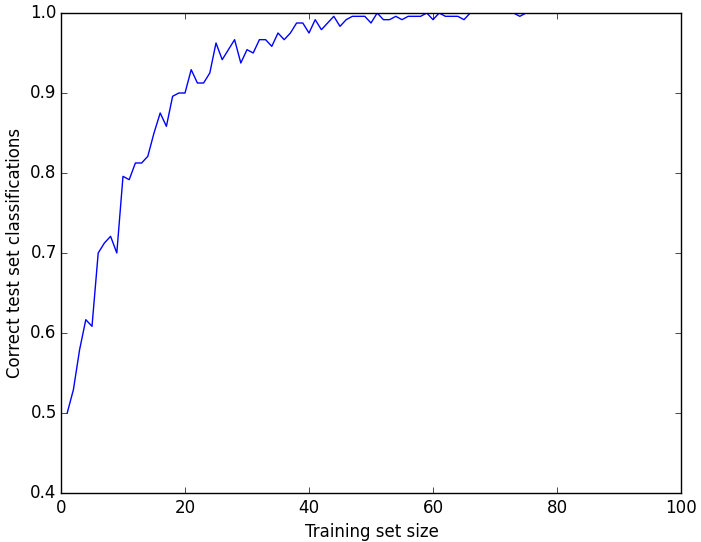
\includegraphics[scale=0.5]{restaurant_learning_curve.png}
    \caption{The dependence on training set size on the test set performance. Examples for the training set were generated via a bootstrap sampling method for 100 examples and averaged over 20 trails (as was done in \cite{Russell}).}
    \label{fig:learning-curve}
\end{figure}


\section{Discussion}

The implementation used in this project produces the same results as those seen in \cite{Russell} for the restaurant example, indicating that the algorithm performs as expected.

We also tried implemented $\chi^2$-pruning but unfortunately we came across problems when trying to prune the restaurant example decision tree. Our implementation suggested pruning the entire tree, which seemed a bit drastic. Therefore the decision was made to drop this feature from the program.


\printbibliography

\end{document}
